\documentclass{ximera}

 

\usepackage{epsfig}

\graphicspath{
  {./}
  {figures/}
}

\usepackage{morewrites}
\makeatletter
\newcommand\subfile[1]{%
\renewcommand{\input}[1]{}%
\begingroup\skip@preamble\otherinput{#1}\endgroup\par\vspace{\topsep}
\let\input\otherinput}
\makeatother

\newcommand{\includeexercises}{\directlua{dofile("/home/jim/linearAlgebra/laode/exercises.lua")}}

%\newcounter{ccounter}
%\setcounter{ccounter}{1}
%\newcommand{\Chapter}[1]{\setcounter{chapter}{\arabic{ccounter}}\chapter{#1}\addtocounter{ccounter}{1}}

%\newcommand{\section}[1]{\section{#1}\setcounter{thm}{0}\setcounter{equation}{0}}

%\renewcommand{\theequation}{\arabic{chapter}.\arabic{section}.\arabic{equation}}
%\renewcommand{\thefigure}{\arabic{chapter}.\arabic{figure}}
%\renewcommand{\thetable}{\arabic{chapter}.\arabic{table}}

%\newcommand{\Sec}[2]{\section{#1}\markright{\arabic{ccounter}.\arabic{section}.#2}\setcounter{equation}{0}\setcounter{thm}{0}\setcounter{figure}{0}}

\newcommand{\Sec}[2]{\section{#1}}

\setcounter{secnumdepth}{2}
%\setcounter{secnumdepth}{1} 

%\newcounter{THM}
%\renewcommand{\theTHM}{\arabic{chapter}.\arabic{section}}

\newcommand{\trademark}{{R\!\!\!\!\!\bigcirc}}
%\newtheorem{exercise}{}

\newcommand{\dfield}{{\sf dfield9}}
\newcommand{\pplane}{{\sf pplane9}}

\newcommand{\EXER}{\section*{Exercises}}%\vspace*{0.2in}\hrule\small\setcounter{exercise}{0}}
\newcommand{\CEXER}{}%\vspace{0.08in}\begin{center}Computer Exercises\end{center}}
\newcommand{\TEXER}{} %\vspace{0.08in}\begin{center}Hand Exercises\end{center}}
\newcommand{\AEXER}{} %\vspace{0.08in}\begin{center}Hand Exercises\end{center}}

% BADBAD: \newcommand{\Bbb}{\bf}

\newcommand{\R}{\mbox{$\Bbb{R}$}}
\newcommand{\C}{\mbox{$\Bbb{C}$}}
\newcommand{\Z}{\mbox{$\Bbb{Z}$}}
\newcommand{\N}{\mbox{$\Bbb{N}$}}
\newcommand{\D}{\mbox{{\bf D}}}
\usepackage{amssymb}
%\newcommand{\qed}{\hfill\mbox{\raggedright$\square$} \vspace{1ex}}
%\newcommand{\proof}{\noindent {\bf Proof:} \hspace{0.1in}}

\newcommand{\setmin}{\;\mbox{--}\;}
\newcommand{\Matlab}{{M\small{AT\-LAB}} }
\newcommand{\Matlabp}{{M\small{AT\-LAB}}}
\newcommand{\computer}{\Matlab Instructions}
\newcommand{\half}{\mbox{$\frac{1}{2}$}}
\newcommand{\compose}{\raisebox{.15ex}{\mbox{{\scriptsize$\circ$}}}}
\newcommand{\AND}{\quad\mbox{and}\quad}
\newcommand{\vect}[2]{\left(\begin{array}{c} #1_1 \\ \vdots \\
 #1_{#2}\end{array}\right)}
\newcommand{\mattwo}[4]{\left(\begin{array}{rr} #1 & #2\\ #3
&#4\end{array}\right)}
\newcommand{\mattwoc}[4]{\left(\begin{array}{cc} #1 & #2\\ #3
&#4\end{array}\right)}
\newcommand{\vectwo}[2]{\left(\begin{array}{r} #1 \\ #2\end{array}\right)}
\newcommand{\vectwoc}[2]{\left(\begin{array}{c} #1 \\ #2\end{array}\right)}

\newcommand{\ignore}[1]{}


\newcommand{\inv}{^{-1}}
\newcommand{\CC}{{\cal C}}
\newcommand{\CCone}{\CC^1}
\newcommand{\Span}{{\rm span}}
\newcommand{\rank}{{\rm rank}}
\newcommand{\trace}{{\rm tr}}
\newcommand{\RE}{{\rm Re}}
\newcommand{\IM}{{\rm Im}}
\newcommand{\nulls}{{\rm null\;space}}

\newcommand{\dps}{\displaystyle}
\newcommand{\arraystart}{\renewcommand{\arraystretch}{1.8}}
\newcommand{\arrayfinish}{\renewcommand{\arraystretch}{1.2}}
\newcommand{\Start}[1]{\vspace{0.08in}\noindent {\bf Section~\ref{#1}}}
\newcommand{\exer}[1]{\noindent {\bf \ref{#1}}}
\newcommand{\ans}{}
\newcommand{\matthree}[9]{\left(\begin{array}{rrr} #1 & #2 & #3 \\ #4 & #5 & #6
\\ #7 & #8 & #9\end{array}\right)}
\newcommand{\cvectwo}[2]{\left(\begin{array}{c} #1 \\ #2\end{array}\right)}
\newcommand{\cmatthree}[9]{\left(\begin{array}{ccc} #1 & #2 & #3 \\ #4 & #5 &
#6 \\ #7 & #8 & #9\end{array}\right)}
\newcommand{\vecthree}[3]{\left(\begin{array}{r} #1 \\ #2 \\
#3\end{array}\right)}
\newcommand{\cvecthree}[3]{\left(\begin{array}{c} #1 \\ #2 \\
#3\end{array}\right)}
\newcommand{\cmattwo}[4]{\left(\begin{array}{cc} #1 & #2\\ #3
&#4\end{array}\right)}

\newcommand{\Matrix}[1]{\ensuremath{\left(\begin{array}{rrrrrrrrrrrrrrrrrr} #1 \end{array}\right)}}

\newcommand{\Matrixc}[1]{\ensuremath{\left(\begin{array}{cccccccccccc} #1 \end{array}\right)}}



\renewcommand{\labelenumi}{\theenumi)}
\newenvironment{enumeratea}%
{\begingroup
 \renewcommand{\theenumi}{\alph{enumi}}
 \renewcommand{\labelenumi}{(\theenumi)}
 \begin{enumerate}}
 {\end{enumerate}\endgroup}



\newcounter{help}
\renewcommand{\thehelp}{\thesection.\arabic{equation}}

%\newenvironment{equation*}%
%{\renewcommand\endequation{\eqno (\theequation)* $$}%
%   \begin{equation}}%
%   {\end{equation}\renewcommand\endequation{\eqno \@eqnnum
%$$\global\@ignoretrue}}

%\input{psfig.tex}

\author{Martin Golubitsky and Michael Dellnitz}

%\newenvironment{matlabEquation}%
%{\renewcommand\endequation{\eqno (\theequation*) $$}%
%   \begin{equation}}%
%   {\end{equation}\renewcommand\endequation{\eqno \@eqnnum
% $$\global\@ignoretrue}}

\newcommand{\soln}{\textbf{Solution:} }
\newcommand{\exercap}[1]{\centerline{Figure~\ref{#1}}}
\newcommand{\exercaptwo}[1]{\centerline{Figure~\ref{#1}a\hspace{2.1in}
Figure~\ref{#1}b}}
\newcommand{\exercapthree}[1]{\centerline{Figure~\ref{#1}a\hspace{1.2in}
Figure~\ref{#1}b\hspace{1.2in}Figure~\ref{#1}c}}
\newcommand{\para}{\hspace{0.4in}}

\renewenvironment{solution}{\suppress}{\endsuppress}

\ifxake
\newenvironment{matlabEquation}{\begin{equation}}{\end{equation}}
\else
\newenvironment{matlabEquation}%
{\let\oldtheequation\theequation\renewcommand{\theequation}{\oldtheequation*}\begin{equation}}%
  {\end{equation}\let\theequation\oldtheequation}
\fi

\makeatother


\title{Phase Space Pictures and Equilibria}

\begin{document}
\begin{abstract}
\end{abstract}
\maketitle

 \label{S:PSP&E}

Recall that in a {\em phase space\/} \index{phase!space} plot, the 
solution $x(t)$ represents the position $x$ of a particle on a line 
for each time $t$.  Phase space plots are difficult to draw, since 
motion must be built into the plot.  However, we can view this 
dynamically in \Matlab using the program {\sf pline}. \index{\computer!pline}

In this discussion, we will only plot solutions of autonomous,
first order differential equations; that is, equations of the
form
\[
\dot{x} = g(x).
\]
To begin, type
\begin{verbatim}
pline
\end{verbatim}
and the window with the {\sf PLINE Setup} appears on the
computer screen.  The layout is essentially the same as in the
{\sf DFIELD5 Setup} described above.  However, there are two
differences:
\begin{enumerate}
\item Since we assume that our equation is autonomous, the time
variable --- the independent variable --- does
not appear explicitly and no time interval is specified.  Rather
the {\sf Integration time}, the period for which the solution is
to be computed, has to be declared.  This change is due to the
convention that all numerical computations start at $t=0$.
\item We may enter equations with one free parameter.
In the {\sf PLINE Setup} that parameter is {\sf lambda}.
Moreover, we may choose the value for that parameter.  The
default value in the {\sf PLINE Setup} is $-0.8$.  Hence, the
default equation used by {\sf pline} is equation
\Ref{lin1} with $\lambda = -0.8$.
\end{enumerate}

When we click with the left mouse button onto the button {\sf
Proceed}, then the display window with the title {\sf PLINE
Display} opens and the $x$-axis shown in Figure~\ref{pl_dsp1}
becomes visible.

\begin{figure}[htb]
     \centerline{%
     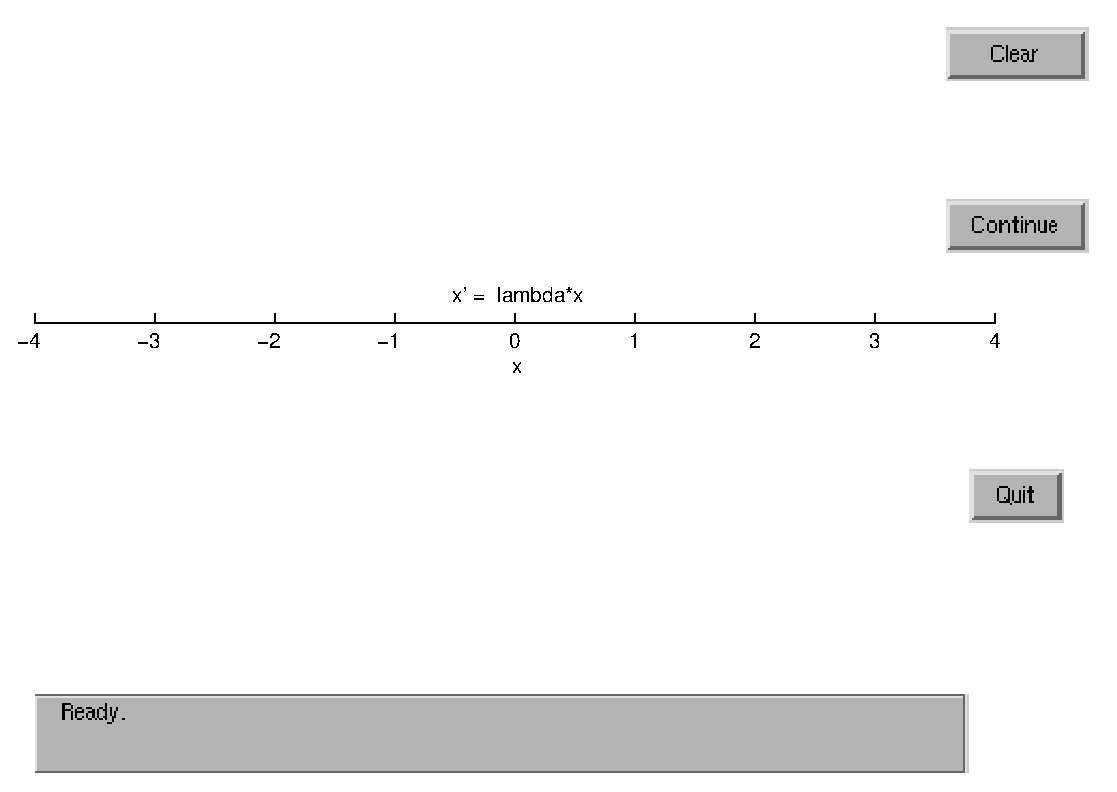
\psfig{file=../figures/pl_dsp1.eps,height=2.6in}}
     \caption{{\sf PLINE Display} for $\dot{x}=\lambda x$
                and $x\in [-4,4]$.}
     \label{pl_dsp1}
\end{figure}

Similar to {\sf dfield5} we may start the numerical solution by
clicking with the left mouse button on the initial value of $x$.
It is not necessary to hit the axis precisely.  For example,
when we click (approximately) on $3$, a colored disk becomes
visible and moves to the left until it stops at a value for $x$
that is between $0.05$ and $0.06$.  This value can be read at
the bottom of the window from the message {\sf Endpoint:
0.05\ldots}.  We can also enter the initial point by choosing
the option {\sf Keyboard input} from the {\sf PLINE Options}
menu.  In fact, if we enter $x=3$ in that window and click on
{\sf Compute}, then the corresponding solution is computed and
we obtain the message {\sf Endpoint: 0.05495}.  Sometimes it
helps to clear all markers in the display window; this is
accomplished by clicking on {\sf Clear}.

\subsection*{Equilibria and Dynamics}

The simplest solution to a differential equation is a solution
that remains constant for all time.  Such solutions are called
{\em equilibria\/}.  Equilibria are found as follows:
\begin{lemma}  \label{L:equilibria}
Consider the autonomous \index{autonomous} differential equation
\begin{equation} \label{aut}
\frac{dx}{dt}(t) = g(x(t)).
\end{equation}
Then $x(t)=x_0$ is an equilibrium \index{equilibrium} if and only
if $g(x_0)=0$.
\end{lemma}

\begin{proof} Suppose that $x(t)=x_0$ is an equilibrium solution to
\Ref{aut}. Then $g(x_0)=0$, since $dx/dt = 0$.  Conversely,
suppose $g(x_0)=0$.  Then $x(t)=x_0$ is a solution to \Ref{aut}.
\end{proof}

We now return to {\sf pline} and the autonomous equation
$g(x)=-0.8x$.  If we continue the integration by pushing {\sf
Continue} in the display window we see again that the solution
approaches $0$ as $t$ goes to infinity; that is, the solution
approaches the equilibrium given by $x(t)=0$.  Correspondingly,
the point that indicates the position of $x(t)$ in the display
window does not move any more.  Solutions that have initial
conditions near $0$ either tend towards $0$ when $\lambda <
0$ or away from $0$ when $\lambda> 0$.

An equilibrium $x(t)=x_0$ is {\em asymptotically stable\/}
\index{stability!asymptotic} if all solutions $y(t)$ with
initial condition $y(0)$ near $x_0$ have the limit
$x_0$ as $t$ goes to infinity.  In symbols we require
\[
\lim_{t\to\infty} y(t) = x_0.
\]
(The definition of asymptotic stability is more complicated in
higher dimensions.) The equilibrium $x(t)=x_0$ is {\em unstable\/}
\index{unstable} if trajectories starting near $x_0$ move away
from $x_0$.  Thus, in
our example, the equilibrium $x=0$ is {\em asymptotically
stable\/} when $\lambda< 0$ and {\em unstable\/}
when $\lambda> 0$.

The dynamical behavior of autonomous differential equations of
the form \Ref{aut} is essentially determined by the equilibria
of $g$.  We explore this statement by using {\sf pline} to
analyze the dynamical behavior of the ordinary differential
equation
\begin{equation} \label{pitch_eq}
	\dot{x} = x(\lambda-x^2),
\end{equation}
where $\lambda$ is a constant.  

First, enter this equation by editing the upper box in the 
{\sf PLINE Setup} window.  Do this editing by clicking in 
the window and deleting the default equation and then type 
{\sf x*(lambda-x\^{$\,\!$}2)}.  Then change the minimum 
and maximum values of $x$ from $-4$ and $4$ to $-2$ and $2$.  
Finally, change the integration time to $1$ and the value
of {\sf lambda} to $-1$.  

Second,  push on {\sf Proceed} so that the $x$ axis becomes 
visible in the display window.
On integrating the system, we find that solutions seem
to behave in a similar way to the solutions of \Ref{lin1} for
$\lambda < 0$: all the solutions approach zero as $t$ goes to
infinity.  Indeed, we can see that $x(t)=0$ is an equilibrium
solution of \Ref{pitch_eq} for all values of $\lambda$.  When
$\lambda<0$ numerical exploration suggests that $0$ is an
asymptotically stable equilibrium.

We now explore the stability properties of $x(t)=0$ when
$\lambda >0$.  We begin by changing the value of $\lambda$ to
$+1$.  We do this in the setup window and afterwards we confirm
the change by pushing {\sf Proceed}.  If we now compute
solutions of the differential equation, then we see that they
come to a rest at $+1$ if we start with a positive value for
$x(0)$ whereas they approach $-1$ if we start with a negative
value for $x(0)$.  Even if we begin the numerical computation
very close to $x=0$, the solutions tend to either $+1$ or $-1$.
These calculations indicate that $0$ is an unstable equilibrium
while both $+1$ and $-1$ are stable equilibria of \Ref{pitch_eq}
when $\lambda =1$.

We use the {\sf Keyboard input} to check that $x(t) = +1$ or
$x(t) = -1$ are equilibrium solutions.  Start the computations
with initial values $x(0) = +1$ or $x(0) = -1$ and see that the
solutions remain constant in time.  Alternatively, solve the
equation
\[
x(1-x^2) = 0,
\]
to see that $x=0,1,-1$ are all equilibria of \Ref{pitch_eq} when
$\lambda=1$.

Our numerical computations indicate that changing the
value of $\lambda$ from $-1$ to $+1$ changes the stability
property of the equilibrium $x(t)=0$.

We can now discuss a method for completely determining the
dynamics of a single autonomous differential equation \Ref{aut}
--- assuming that equilibria are isolated.

\begin{itemize}
\item Determine all equilibria of \Ref{aut} by solving the
equation $g(x)=0$.
\item Choose an initial point between each pair of consecutive
equilibria and determine the direction of motion (sign of $g$) at
that initial point. This can be done either directly or by using
{\sf pline}.
\item On a line plot the equilibria \index{equilibrium} and
connect them by arrows indicating the direction of the dynamics.
\end{itemize}
For example, the dynamics of the differential equations $\dot{x}
= x(-1-x^2)$ and $\dot{x} = x(1-x^2)$ are shown schematically in
Figure~\ref{pitch3}.

\begin{figure}[htb]
       \centerline{%
	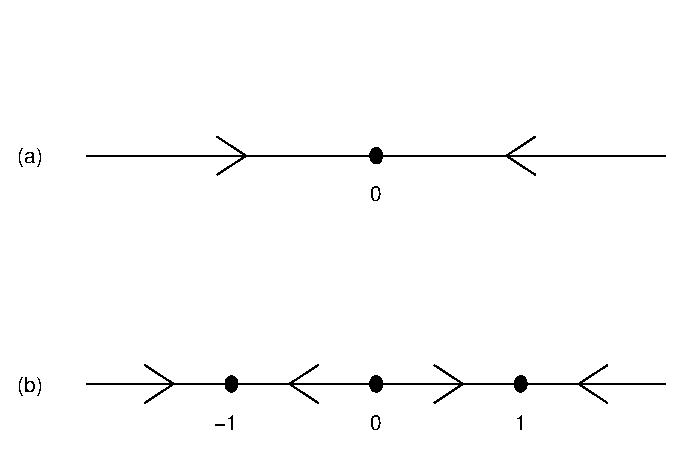
\psfig{file=../figures/schemdyn.eps,width=3.4in}}
\caption{Schematic dynamics of (a) $\dot{x}=x(-1-x^2)$ and (b) $\dot{x}=x(1-x^2)$.}
\label{pitch3}
\end{figure}

\subsubsection*{Hyperbolic Equilibria}

Suppose that $x_0$ is an equilibrium for \Ref{aut}; that is suppose
$g(x_0)=0$.  We denote the derivative of $g(x)$ with respect to $x$, 
$dg/dx$, by $g'$.  The equilibrium $x_0$ is 
{\em hyperbolic\/} \index{hyperbolic}
if $g'(x_0)\neq 0$.  Assume that $x_0$ is a hyperbolic equilibrium and use
the tangent line approximation to $g(x)$ near $x_0$
($\Delta g = g'(x_0)\Delta x$) and that fact that $g(x_0)=0$ to conclude that
\[
g(x) \approx g'(x_0)(x-x_0).
\]
It follows that if $g'(x_0)<0$, then $g(x)$ is negative when
$x>x_0$ and positive when $x<x_0$.  So when $g'(x_0)<0$,
solutions of \Ref{aut} starting just to the right of $x_0$ will
move left ($g<0$) and tend towards $x_0$ and solutions starting
just to the left of $x_0$ will move right ($g>0$) and tend
towards $x_0$.  Similarly, if $g'(x_0)>0$, then $g(x)$ is positive
when $x>x_0$ and negative when $x<x_0$.  Thus, solutions near $x_0$ 
will tend away from $x_0$ when $g'(x_0)>0$.    We  have shown:
\begin{theorem}[Stability of Hyperbolic Equilibria] \label{T:stability1}
Let $x_0$ be a hyperbolic equilibrium for the differential equation
\[
\frac{dx}{dt} = g(x).
\]
If $g'(x_0)<0$, then the equilibrium is asymptotically stable;
and if $g'(x_0)>0$, then the equilibrium is unstable.
\end{theorem} \index{equilibrium} \index{stability!asymptotic}
\index{unstable}

It follows from Theorem~\ref{T:stability1} that the phase line picture
near a hyperbolic equilibrium is particularly simple as the arrows beside
that equilibrium either both point towards the equilibrium (as in
Figure~\ref{pitch3}(a)) or both point away from the equilibrium (as near $0$
in Figure~\ref{pitch3}(b)).

\subsection*{Comparing Phase Lines and Time Series}
\index{phase!line}\index{time series}

Phase line plots and time series graphs give different ways of
presenting the same information.  With that point in mind, it is
important to be able to recreate one type of plot from
the other.  For example, let $x(t)$ be the solution to the
differential equation $\dot{x}=x(1-x^2)$ with initial condition $x(0)=2$.
In Figure~\ref{pitch3}(b) we have drawn the schematic phase line for
all solutions to this differential equation. How can we reconstruct
a (schematic) graph of the time series $x(t)$ for this solution just
from the phase line?

To answer this question, note that in Figure~\ref{pitch3}(b) the
initial condition $x(0)=2$ lies to the right of all equilibria of
this equation, and the arrow indicates that solution trajectories
starting in this area move to the left, that is, they decrease to
the equilibrium at $x=1$.  It follows that
\[
\lim_{t\to\infty} x(t) = 1.
\]
Since there are no equilibria to the right of $x=2$, the graph of $x(t)$
must increase to infinity in {\em backwards\/} time.  So the graph of 
$x=x(t)$ is decreasing and asymptotic to $x=1$ for large positive $t$.  
A schematic graph is given in Figure~\ref{pitch3a}(a).  Using {\sf dfield5} 
we can check this description by numerically integrating the differential
equation.   This graph is shown in Figure~\ref{pitch3a}(b).

\begin{figure}[htb]
       \centerline{%
        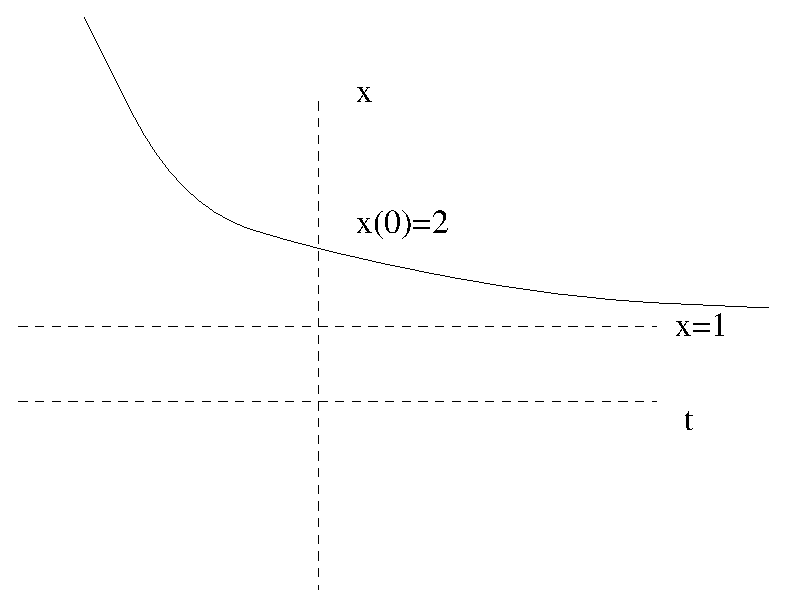
\psfig{file=../figures/pitch3as.eps,width=2.8in}
	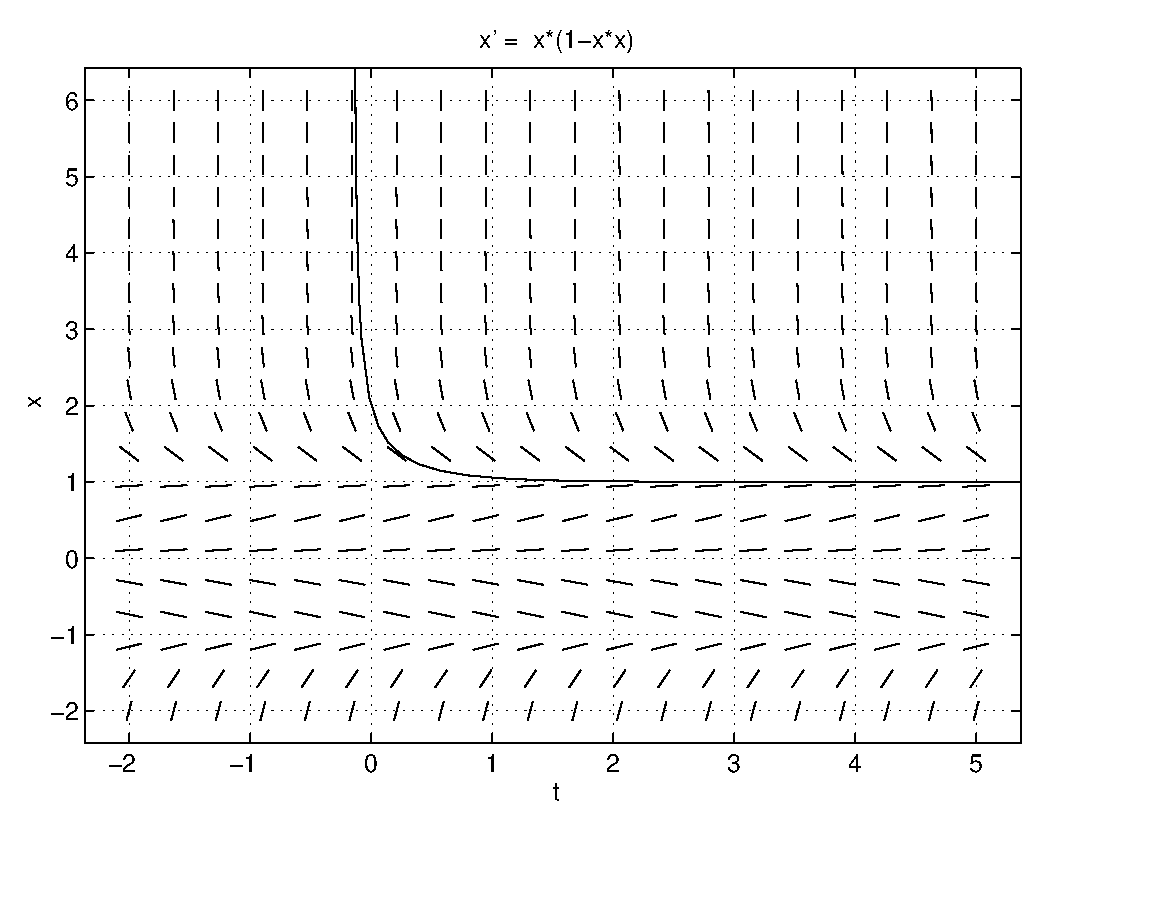
\psfig{file=../figures/pitch3ad.eps,width=3.0in}}
       \caption{Time series for solution to $\dot{x}=x(1-x^2)$ with $x(0)=2$.
	(Left) Sketch using asymptotic information; (right) {\sf dfield5}
	computation.}
       \label{pitch3a}
\end{figure}



\EXER

\CEXER

\begin{exercise} \label{c3.3.1}
Use {\sf pline} to find an initial condition $x(0)$ for the
ordinary differential equation \Ref{lin1} with $\lambda=-0.2$
such that the corresponding solution $x(t)$ satisfies
$x(20)\in[0.001,0.002]$.
\end{exercise}

\begin{exercise} \label{c3.3.2}
Use {\sf pline} to find all the equilibria of the ordinary
differential equation
\[
\dot{x} = (x^2-1)(x+2).
\]
Which of the equilibria are stable and which are unstable?
\end{exercise}

\begin{exercise} \label{c3.3.3}
Consider the following ordinary differential equation:
\[
\dot{x} = \lambda x(1-x).
\]
Use {\sf pline} to find a value for the parameter $\lambda$ such
that $x(t)=1$ is a stable equilibrium.
\end{exercise}

\begin{exercise} \label{c3.3.4}
The differential equation
\[
\frac{dx}{dt} =  x^2
\]
has an equilibrium at the origin.  Use {\sf pline} to determine
those $x_0$ for which solutions to the initial value $x(0)=x_0$ tend
towards the origin.
\end{exercise}

\begin{exercise} \label{c3.3.5}
Consider the differential equation
\[
\frac{dx}{dt} = a x^3.
\]
Use {\sf pline} to verify that the origin is an asymptotically
stable equilibrium when $a = -1$ and is an unstable
equilibrium when $a = +1$. Discuss the relationship
between these examples and Theorem~\ref{T:stability1}.
\end{exercise}

\TEXER


\noindent In Exercises~\ref{c3.3.6A} -- \ref{c3.3.6D} compute the equilibria 
of the given differential equation, determine whether these equilibria are 
asymptotically stable or unstable, and draw a sche\-ma\-tic of the dynamics 
of this equation like the one in Figure~\ref{pitch3}.  You may use {\sf pline}
to check your answer.
\begin{exercise} \label{c3.3.6A}
$\dot{x} = x^2 + 2x - 3$.
\end{exercise}
\begin{exercise} \label{c3.3.6B}
$\dot{x} = x^3 - 2x^2 - 8x$.
\end{exercise}
\begin{exercise} \label{c3.3.6C}
$\dot{x} = x^3 + 2x^2 - 3x$.
\end{exercise}
\begin{exercise} \label{c3.3.6D}
$\dot{x} = x^2 + 6x + 1$.
\end{exercise}

\begin{exercise} \label{c3.3.7}
Let $x(t)$ be a solution to the initial value problem
\begin{eqnarray*}
\dot{x} & = & g(x) \\
x(0) & = & x_0.
\end{eqnarray*}
Let $y(t)=x(-t)$.  Show that $y(t)$ is a solution to the
initial value problem
\begin{eqnarray*}
\dot{y} & = & -g(y) \\
y(0) & = & x_0.
\end{eqnarray*}
(Thus, to integrate the solution $x(t)$ backwards in time is the
same as solving the differential equation $\dot{y}  =  -g(y)$
forward in time.)
\end{exercise}

\begin{exercise} \label{c3.3.9}
Use Exercise~\ref{c3.3.7} to devise a shortcut for solving
Exercise~\ref{c3.3.1}.
\end{exercise}

\begin{exercise} \label{c3.3.8}
Sketch the time series for the solution to the differential
equation pictured in Figure~\ref{pitch3}(b) with initial condition
$x(0)=\frac{1}{2}$.  Use only the phase space plot given in this
figure.  Use {\sf dfield5} to verify your answer.
\end{exercise}

\noindent In Exercises~\ref{c3.3.10a} -- \ref{c3.3.10d} use the line field 
given in Figure~\ref{F:exer3ad} to answer the following:\\
\noindent (a) Is the differential equation that was used to draw this figure 
autonomous or nonautonomous.\\
\noindent (b)  If the differential equation is autonomous, then draw the phase
line noting the values of $x$ where equilibria occur and whether they are 
asymptotically stable or not. If the differential equation is nonautonomous, 
then draw the time series for solutions with initial conditions $x(0)=0$ and 
$x(2)=0$.

\begin{exercise} \label{c3.3.10a}
Use Figure~\ref{F:exer3ad}(i) to answer parts (a) and (b).
\end{exercise}
\begin{exercise} \label{c3.3.10b}
Use Figure~\ref{F:exer3ad}(ii) to answer parts (a) and (b).
\end{exercise}
\begin{exercise} \label{c3.3.10c}
Use Figure~\ref{F:exer3ad}(iii) to answer parts (a) and (b).
\end{exercise}
\begin{exercise} \label{c3.3.10d}
Use Figure~\ref{F:exer3ad}(iv) to answer parts (a) and (b).
\end{exercise}

\begin{figure}[htb]
       \centerline{%
        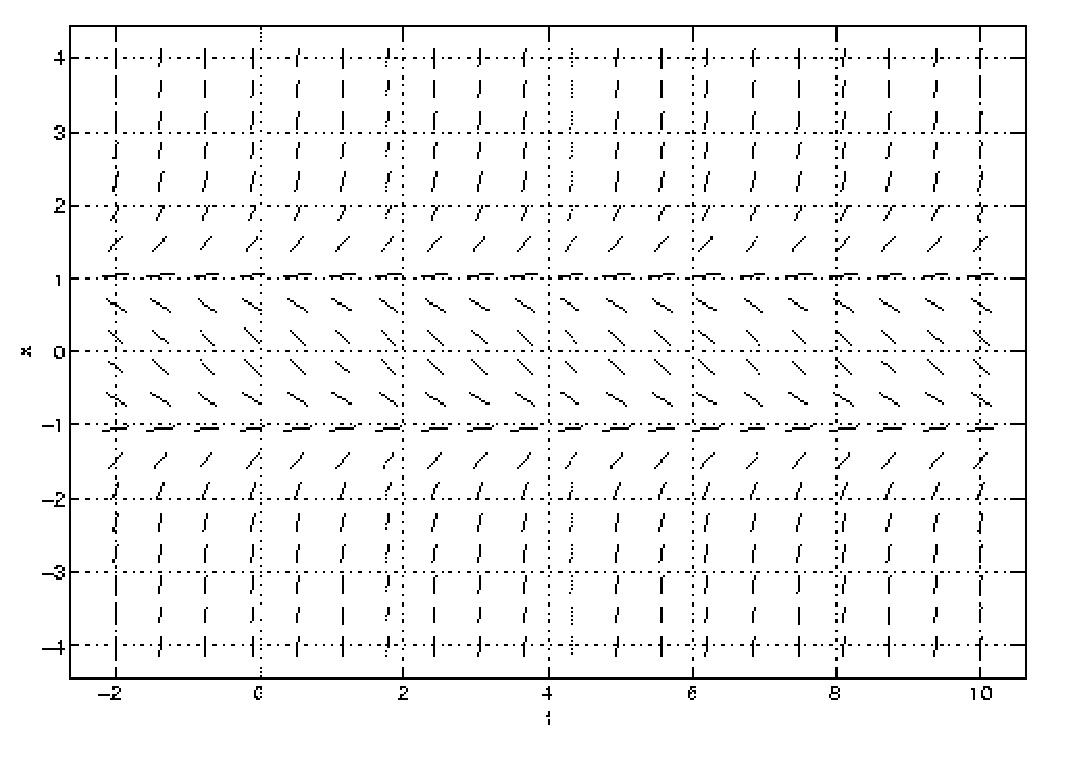
\psfig{file=../figures/auto1a.eps,width=2.8in}
	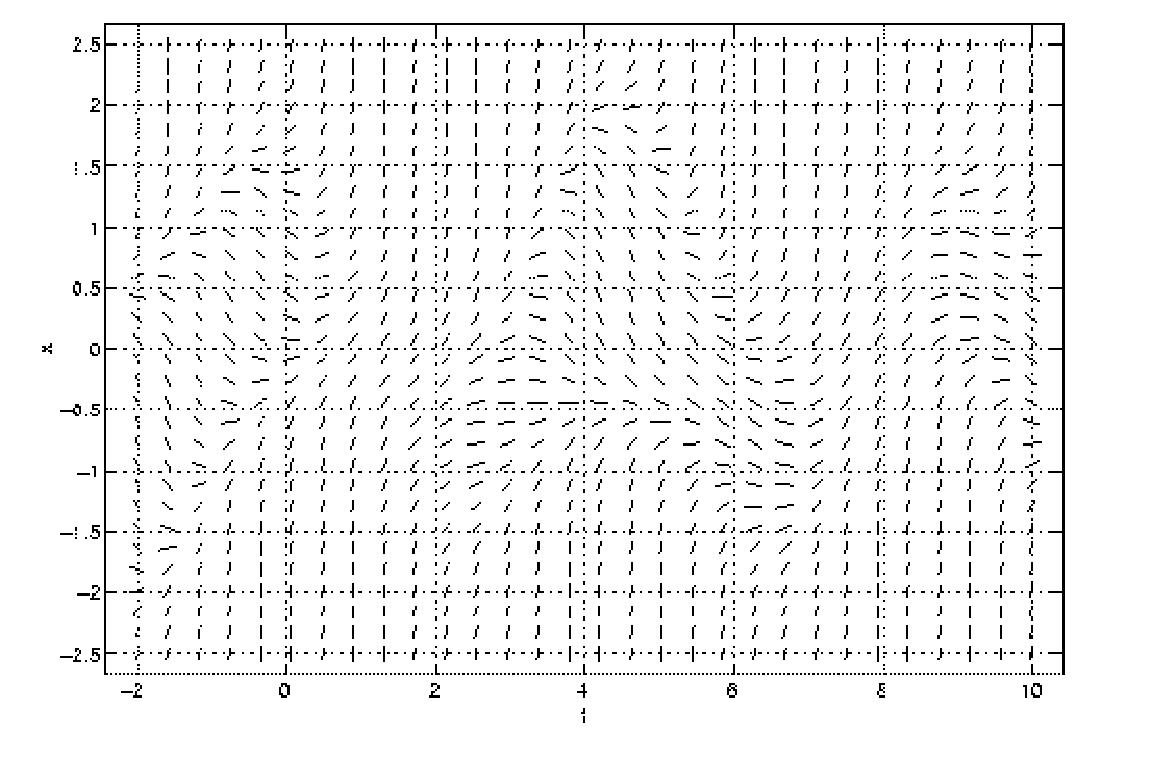
\psfig{file=../figures/nonauto2a.eps,width=2.8in}}
\centerline{(i) \hspace{2.6in} (ii)}
       \centerline{%
        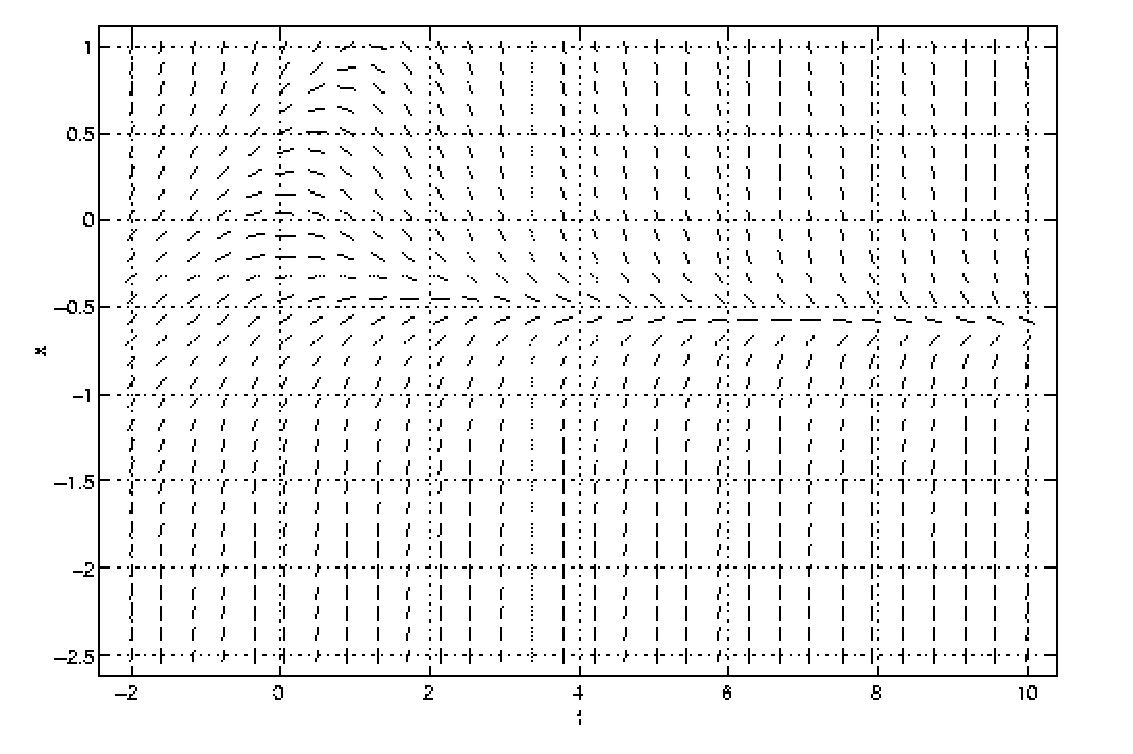
\psfig{file=../figures/nonauto1a.eps,width=2.8in}
	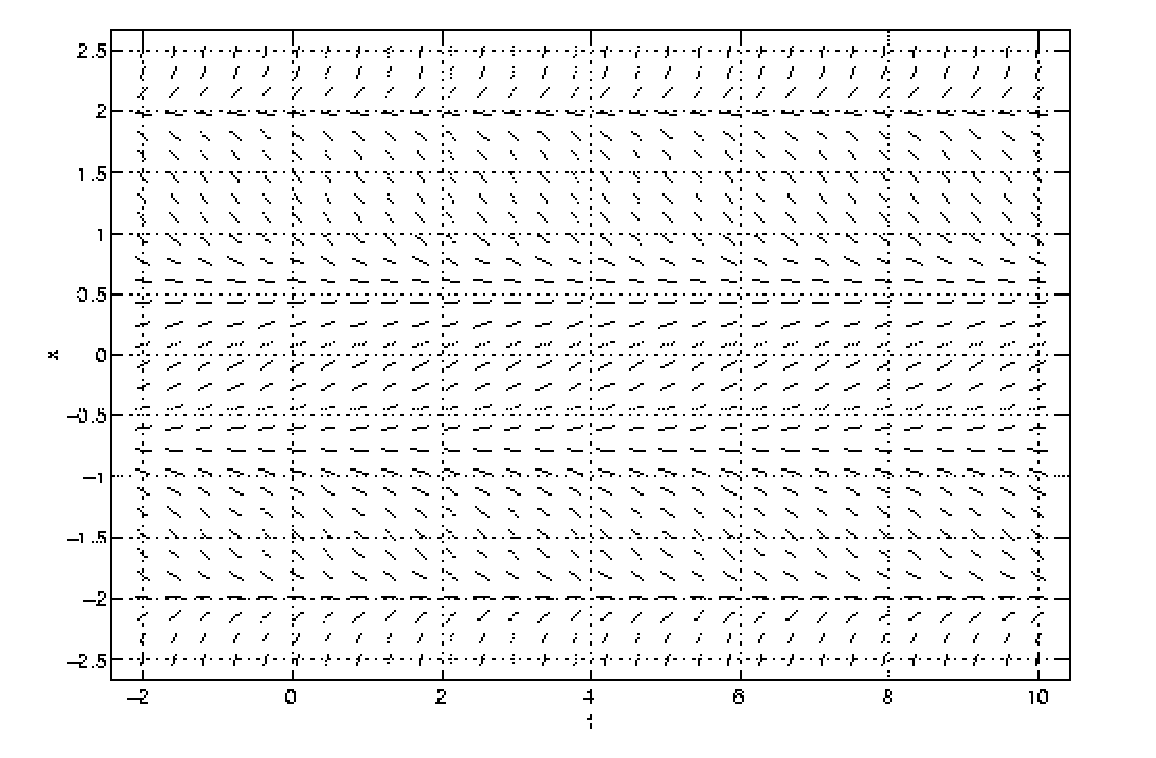
\psfig{file=../figures/auto2a.eps,width=2.8in}}
\centerline{(iii) \hspace{2.6in} (iv)}
       \caption{Figures for Exercises~\protect{\ref{c3.3.10a}} --
\protect{\ref{c3.3.10d}}}
       \label{F:exer3ad}
\end{figure}


\end{document}
